% Options for packages loaded elsewhere
\PassOptionsToPackage{unicode}{hyperref}
\PassOptionsToPackage{hyphens}{url}
%
\documentclass[
]{article}
\usepackage{amsmath,amssymb}
\usepackage{lmodern}
\usepackage{ifxetex,ifluatex}
\ifnum 0\ifxetex 1\fi\ifluatex 1\fi=0 % if pdftex
  \usepackage[T1]{fontenc}
  \usepackage[utf8]{inputenc}
  \usepackage{textcomp} % provide euro and other symbols
\else % if luatex or xetex
  \usepackage{unicode-math}
  \defaultfontfeatures{Scale=MatchLowercase}
  \defaultfontfeatures[\rmfamily]{Ligatures=TeX,Scale=1}
\fi
% Use upquote if available, for straight quotes in verbatim environments
\IfFileExists{upquote.sty}{\usepackage{upquote}}{}
\IfFileExists{microtype.sty}{% use microtype if available
  \usepackage[]{microtype}
  \UseMicrotypeSet[protrusion]{basicmath} % disable protrusion for tt fonts
}{}
\makeatletter
\@ifundefined{KOMAClassName}{% if non-KOMA class
  \IfFileExists{parskip.sty}{%
    \usepackage{parskip}
  }{% else
    \setlength{\parindent}{0pt}
    \setlength{\parskip}{6pt plus 2pt minus 1pt}}
}{% if KOMA class
  \KOMAoptions{parskip=half}}
\makeatother
\usepackage{xcolor}
\IfFileExists{xurl.sty}{\usepackage{xurl}}{} % add URL line breaks if available
\IfFileExists{bookmark.sty}{\usepackage{bookmark}}{\usepackage{hyperref}}
\hypersetup{
  pdftitle={R journal examples},
  hidelinks,
  pdfcreator={LaTeX via pandoc}}
\urlstyle{same} % disable monospaced font for URLs
\usepackage[margin=1in]{geometry}
\usepackage{color}
\usepackage{fancyvrb}
\newcommand{\VerbBar}{|}
\newcommand{\VERB}{\Verb[commandchars=\\\{\}]}
\DefineVerbatimEnvironment{Highlighting}{Verbatim}{commandchars=\\\{\}}
% Add ',fontsize=\small' for more characters per line
\usepackage{framed}
\definecolor{shadecolor}{RGB}{248,248,248}
\newenvironment{Shaded}{\begin{snugshade}}{\end{snugshade}}
\newcommand{\AlertTok}[1]{\textcolor[rgb]{0.94,0.16,0.16}{#1}}
\newcommand{\AnnotationTok}[1]{\textcolor[rgb]{0.56,0.35,0.01}{\textbf{\textit{#1}}}}
\newcommand{\AttributeTok}[1]{\textcolor[rgb]{0.77,0.63,0.00}{#1}}
\newcommand{\BaseNTok}[1]{\textcolor[rgb]{0.00,0.00,0.81}{#1}}
\newcommand{\BuiltInTok}[1]{#1}
\newcommand{\CharTok}[1]{\textcolor[rgb]{0.31,0.60,0.02}{#1}}
\newcommand{\CommentTok}[1]{\textcolor[rgb]{0.56,0.35,0.01}{\textit{#1}}}
\newcommand{\CommentVarTok}[1]{\textcolor[rgb]{0.56,0.35,0.01}{\textbf{\textit{#1}}}}
\newcommand{\ConstantTok}[1]{\textcolor[rgb]{0.00,0.00,0.00}{#1}}
\newcommand{\ControlFlowTok}[1]{\textcolor[rgb]{0.13,0.29,0.53}{\textbf{#1}}}
\newcommand{\DataTypeTok}[1]{\textcolor[rgb]{0.13,0.29,0.53}{#1}}
\newcommand{\DecValTok}[1]{\textcolor[rgb]{0.00,0.00,0.81}{#1}}
\newcommand{\DocumentationTok}[1]{\textcolor[rgb]{0.56,0.35,0.01}{\textbf{\textit{#1}}}}
\newcommand{\ErrorTok}[1]{\textcolor[rgb]{0.64,0.00,0.00}{\textbf{#1}}}
\newcommand{\ExtensionTok}[1]{#1}
\newcommand{\FloatTok}[1]{\textcolor[rgb]{0.00,0.00,0.81}{#1}}
\newcommand{\FunctionTok}[1]{\textcolor[rgb]{0.00,0.00,0.00}{#1}}
\newcommand{\ImportTok}[1]{#1}
\newcommand{\InformationTok}[1]{\textcolor[rgb]{0.56,0.35,0.01}{\textbf{\textit{#1}}}}
\newcommand{\KeywordTok}[1]{\textcolor[rgb]{0.13,0.29,0.53}{\textbf{#1}}}
\newcommand{\NormalTok}[1]{#1}
\newcommand{\OperatorTok}[1]{\textcolor[rgb]{0.81,0.36,0.00}{\textbf{#1}}}
\newcommand{\OtherTok}[1]{\textcolor[rgb]{0.56,0.35,0.01}{#1}}
\newcommand{\PreprocessorTok}[1]{\textcolor[rgb]{0.56,0.35,0.01}{\textit{#1}}}
\newcommand{\RegionMarkerTok}[1]{#1}
\newcommand{\SpecialCharTok}[1]{\textcolor[rgb]{0.00,0.00,0.00}{#1}}
\newcommand{\SpecialStringTok}[1]{\textcolor[rgb]{0.31,0.60,0.02}{#1}}
\newcommand{\StringTok}[1]{\textcolor[rgb]{0.31,0.60,0.02}{#1}}
\newcommand{\VariableTok}[1]{\textcolor[rgb]{0.00,0.00,0.00}{#1}}
\newcommand{\VerbatimStringTok}[1]{\textcolor[rgb]{0.31,0.60,0.02}{#1}}
\newcommand{\WarningTok}[1]{\textcolor[rgb]{0.56,0.35,0.01}{\textbf{\textit{#1}}}}
\usepackage{graphicx}
\makeatletter
\def\maxwidth{\ifdim\Gin@nat@width>\linewidth\linewidth\else\Gin@nat@width\fi}
\def\maxheight{\ifdim\Gin@nat@height>\textheight\textheight\else\Gin@nat@height\fi}
\makeatother
% Scale images if necessary, so that they will not overflow the page
% margins by default, and it is still possible to overwrite the defaults
% using explicit options in \includegraphics[width, height, ...]{}
\setkeys{Gin}{width=\maxwidth,height=\maxheight,keepaspectratio}
% Set default figure placement to htbp
\makeatletter
\def\fps@figure{htbp}
\makeatother
\setlength{\emergencystretch}{3em} % prevent overfull lines
\providecommand{\tightlist}{%
  \setlength{\itemsep}{0pt}\setlength{\parskip}{0pt}}
\setcounter{secnumdepth}{-\maxdimen} % remove section numbering
\ifluatex
  \usepackage{selnolig}  % disable illegal ligatures
\fi

\title{R journal examples}
\author{}
\date{\vspace{-2.5em}}

\begin{document}
\maketitle

\hypertarget{vaccine-data}{%
\subsection{Vaccine data}\label{vaccine-data}}

\begin{Shaded}
\begin{Highlighting}[]
\FunctionTok{data}\NormalTok{ (Vaccine)}

\NormalTok{treats }\OtherTok{\textless{}{-}} \FunctionTok{c}\NormalTok{(}\StringTok{"Status quo"}\NormalTok{, }\StringTok{"Vaccination"}\NormalTok{)}
\NormalTok{bcea\_vacc }\OtherTok{\textless{}{-}} \FunctionTok{bcea}\NormalTok{(e, c, }\AttributeTok{ref =} \DecValTok{2}\NormalTok{, }\AttributeTok{interventions =}\NormalTok{ treats)}
\end{Highlighting}
\end{Shaded}

\begin{Shaded}
\begin{Highlighting}[]
\FunctionTok{plot}\NormalTok{(bcea\_vacc)}
\end{Highlighting}
\end{Shaded}

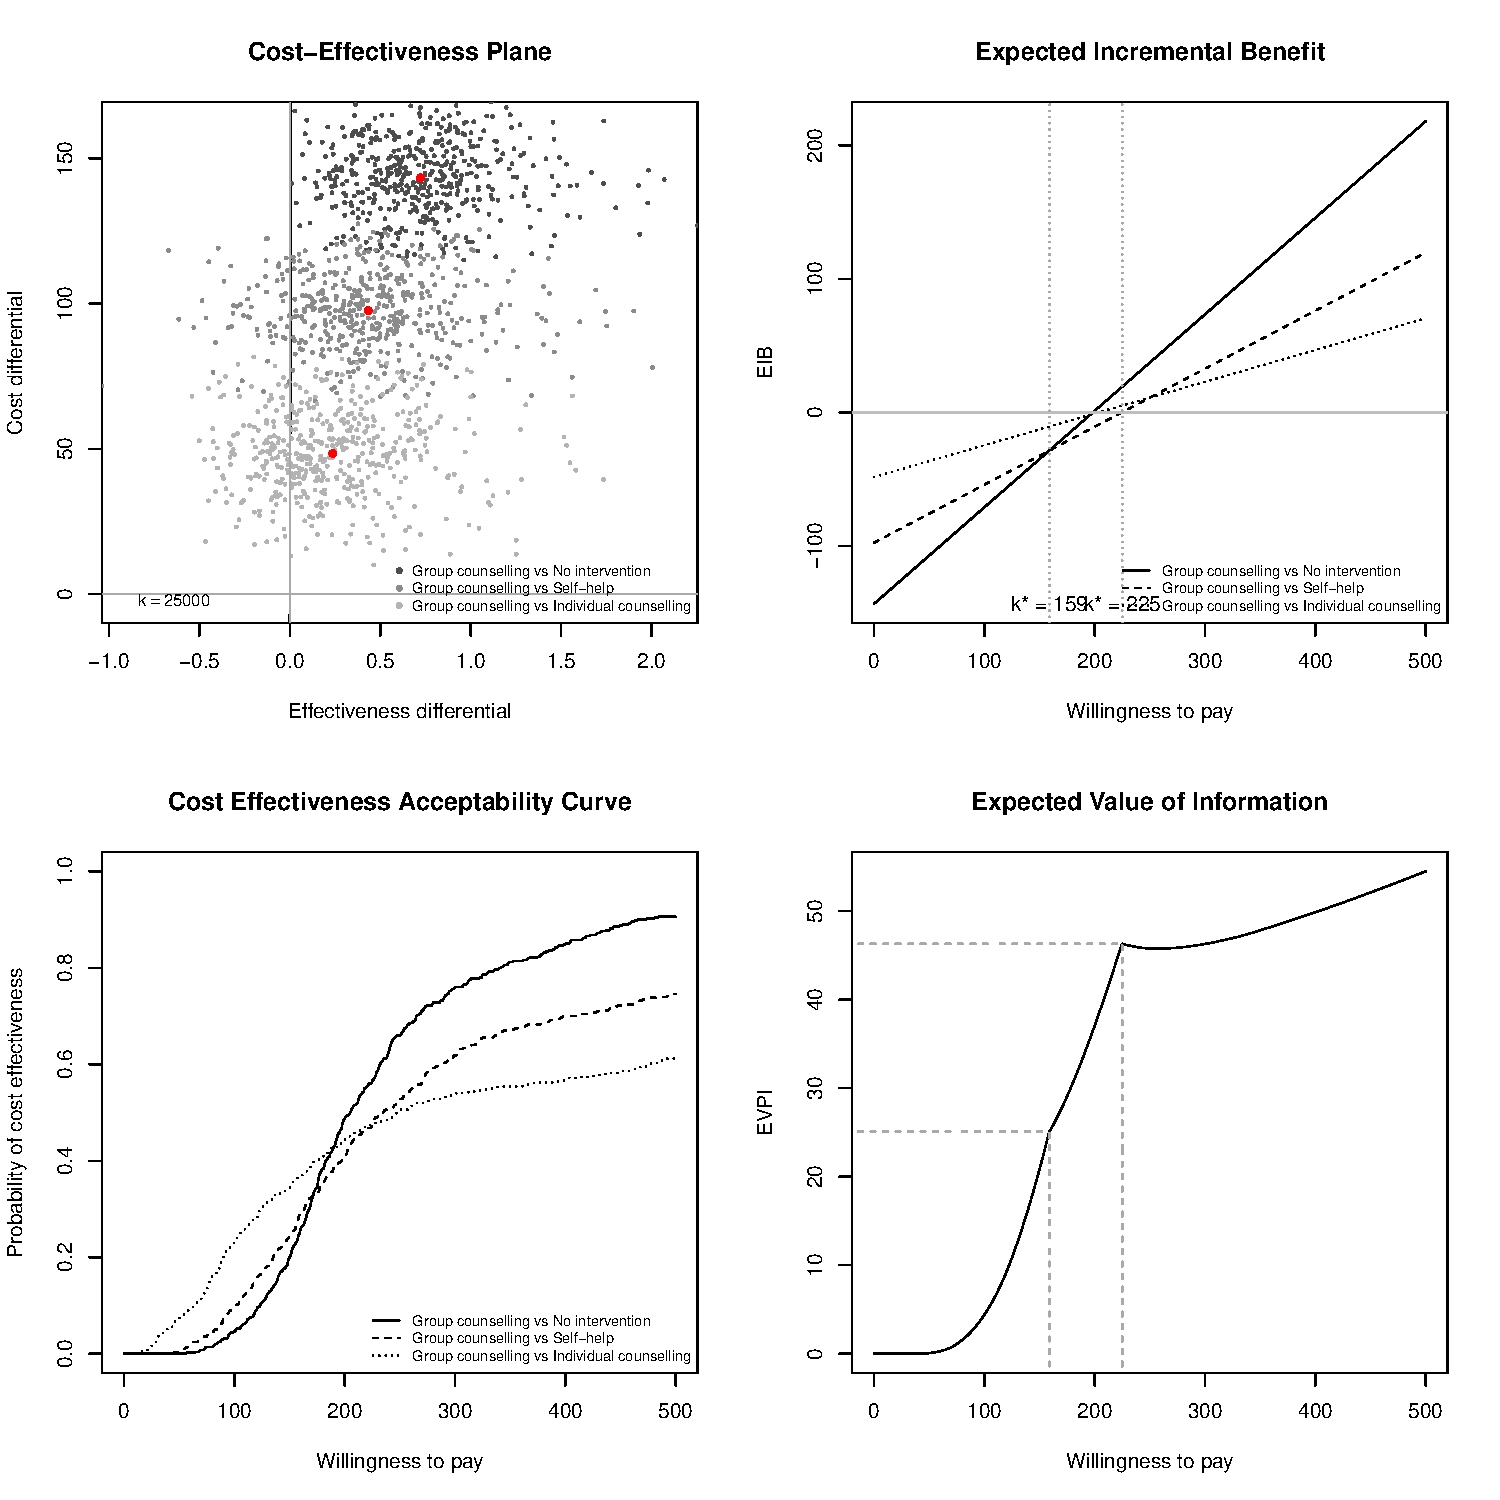
\includegraphics{C:/Users/Nathan/Documents/R/BCEA/vignettes/R_journal_examples_files/figure-latex/unnamed-chunk-4-1.pdf}

\hypertarget{smoking-example}{%
\subsection{Smoking example}\label{smoking-example}}

\begin{Shaded}
\begin{Highlighting}[]
\FunctionTok{data}\NormalTok{(Smoking)}

\NormalTok{treats }\OtherTok{\textless{}{-}} \FunctionTok{c}\NormalTok{(}\StringTok{"No intervention"}\NormalTok{, }\StringTok{"Self{-}help"}\NormalTok{, }\StringTok{"Individual counselling"}\NormalTok{, }\StringTok{"Group counselling"}\NormalTok{)}
\NormalTok{bcea\_smoke }\OtherTok{\textless{}{-}} \FunctionTok{bcea}\NormalTok{(e, c, }\AttributeTok{ref =} \DecValTok{4}\NormalTok{, }\AttributeTok{interventions =}\NormalTok{ treats, }\AttributeTok{Kmax =} \DecValTok{500}\NormalTok{)}
\end{Highlighting}
\end{Shaded}

\begin{Shaded}
\begin{Highlighting}[]
\FunctionTok{plot}\NormalTok{(bcea\_smoke)}
\CommentTok{\#\textgreater{} Wrong number of colours provided. Falling back to default}
\end{Highlighting}
\end{Shaded}

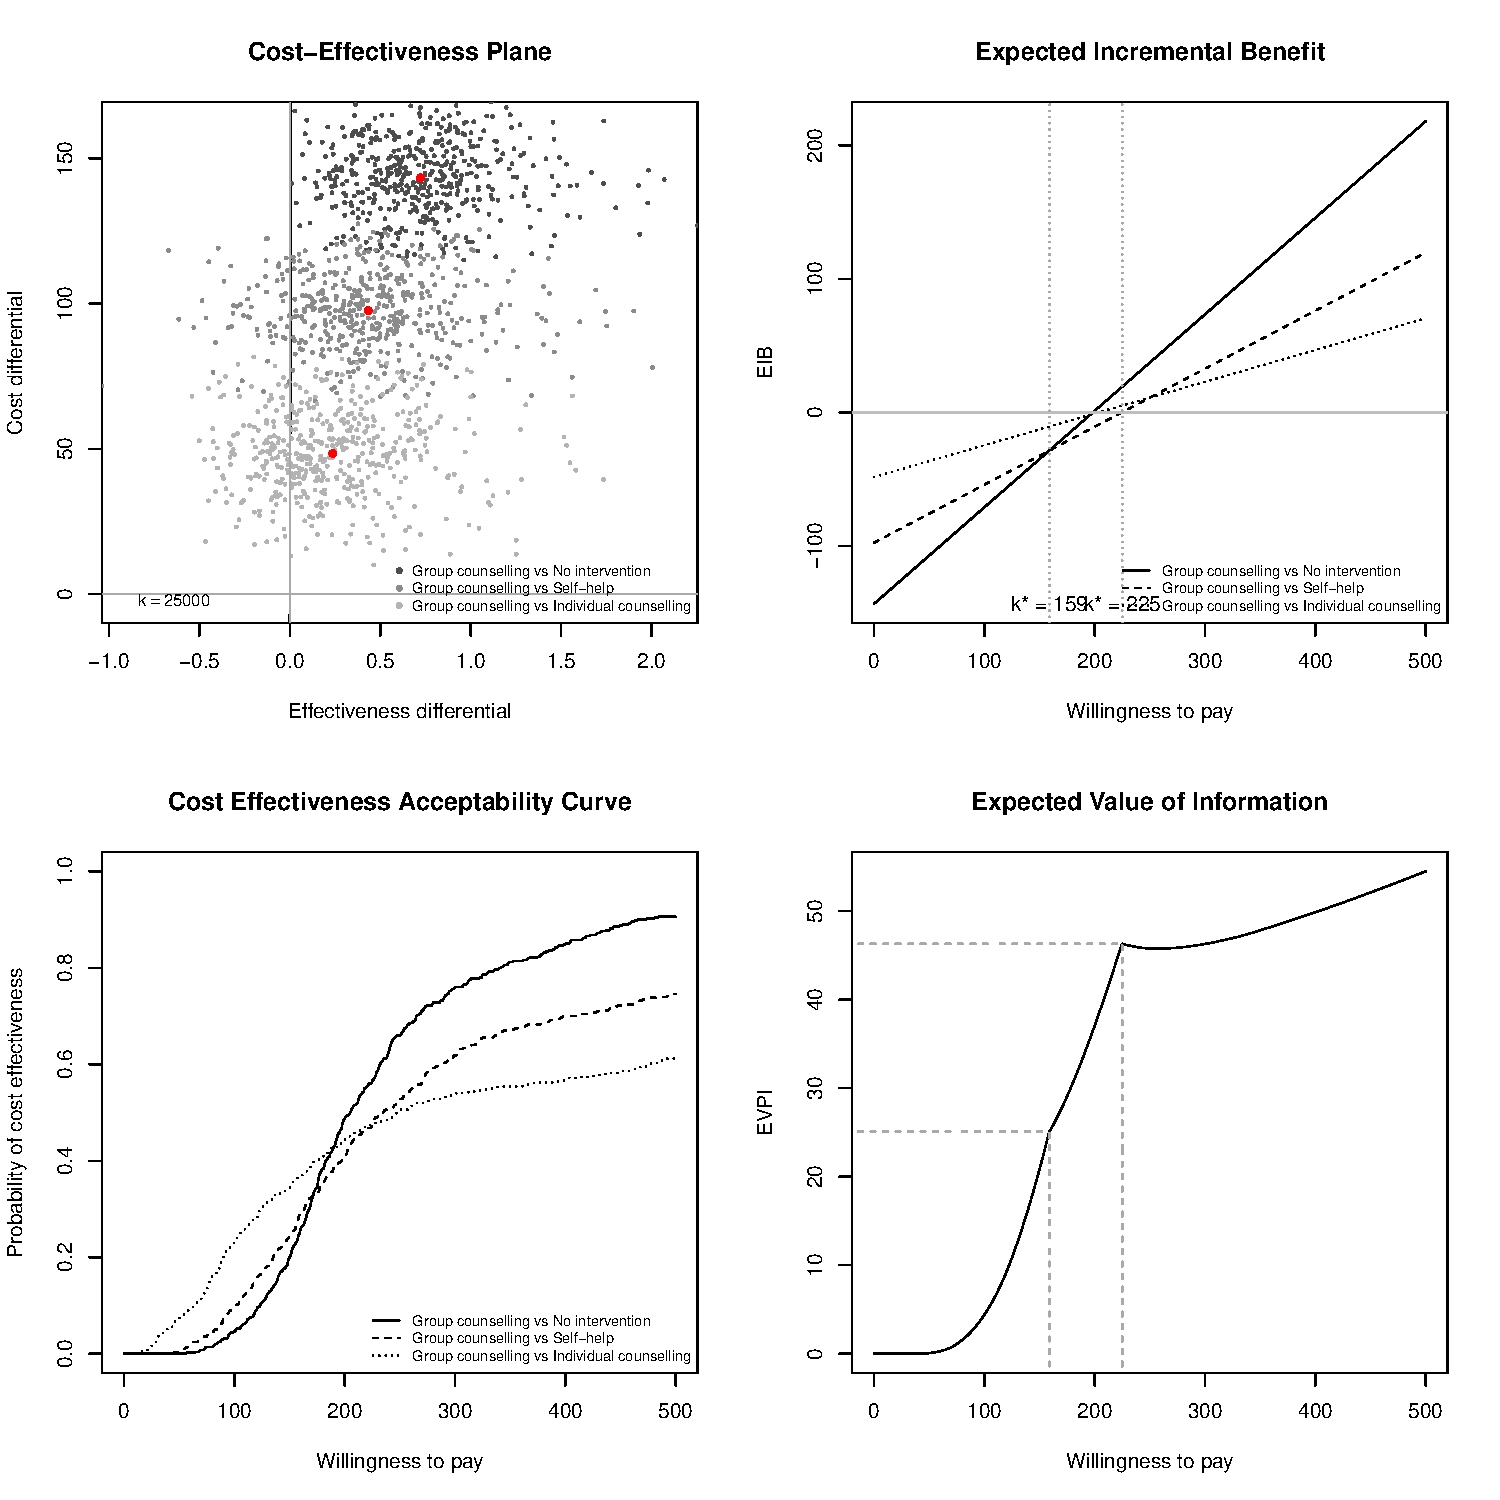
\includegraphics{C:/Users/Nathan/Documents/R/BCEA/vignettes/R_journal_examples_files/figure-latex/plot_bcea_smoke-1.pdf}

\begin{Shaded}
\begin{Highlighting}[]
\NormalTok{bcea\_smoke2 }\OtherTok{\textless{}{-}} \FunctionTok{bcea}\NormalTok{(e, c, }\AttributeTok{ref =} \DecValTok{4}\NormalTok{, }\AttributeTok{wtp =} \FunctionTok{c}\NormalTok{(}\DecValTok{20000}\NormalTok{, }\DecValTok{25000}\NormalTok{, }\DecValTok{30000}\NormalTok{))}
\end{Highlighting}
\end{Shaded}

\begin{Shaded}
\begin{Highlighting}[]
\CommentTok{\# plot(bcea\_smoke2)}
\end{Highlighting}
\end{Shaded}

\begin{Shaded}
\begin{Highlighting}[]
\FunctionTok{library}\NormalTok{(ggplot2)}

\FunctionTok{plot}\NormalTok{(bcea\_smoke, }\AttributeTok{graph =} \StringTok{"ggplot2"}\NormalTok{, }\AttributeTok{wtp =} \DecValTok{250}\NormalTok{, }\AttributeTok{pos =} \ConstantTok{TRUE}\NormalTok{, }\AttributeTok{size =} \FunctionTok{rel}\NormalTok{(}\DecValTok{2}\NormalTok{), }\AttributeTok{ICER.size =} \DecValTok{2}\NormalTok{)}
\end{Highlighting}
\end{Shaded}

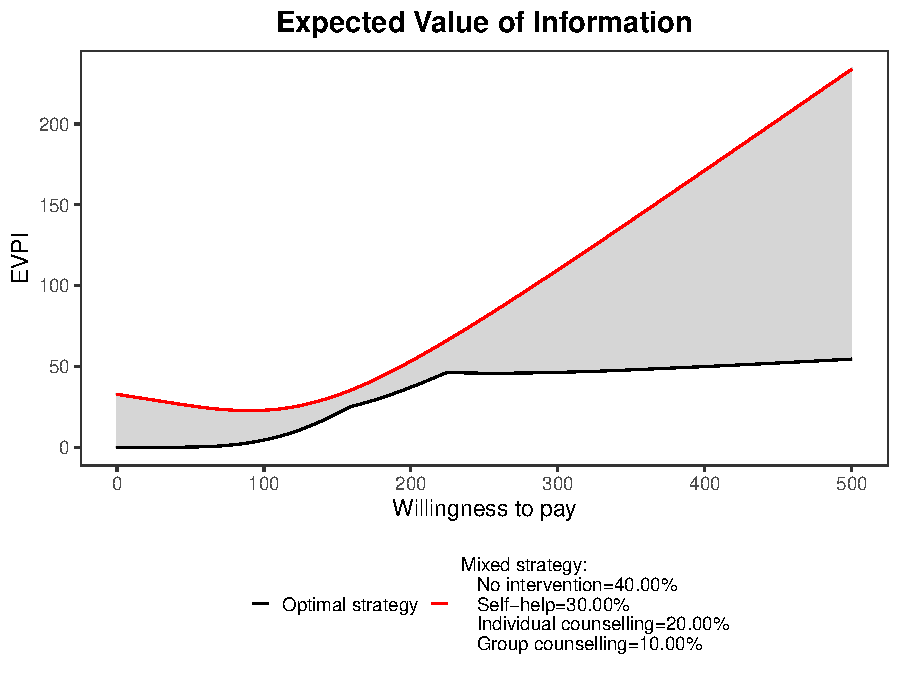
\includegraphics{C:/Users/Nathan/Documents/R/BCEA/vignettes/R_journal_examples_files/figure-latex/unnamed-chunk-8-1.pdf}

\begin{Shaded}
\begin{Highlighting}[]
\CommentTok{\# plot(bcea\_smoke2, graph = "ggplot2")}
\CommentTok{\# when providing wtp to bcea, kstar is NA??...}
\end{Highlighting}
\end{Shaded}

\begin{Shaded}
\begin{Highlighting}[]
\FunctionTok{summary}\NormalTok{(bcea\_smoke, }\AttributeTok{wtp =} \DecValTok{10000}\NormalTok{)}
\CommentTok{\#\textgreater{} NB: k (wtp) is defined in the interval [0 {-} 500]}
\CommentTok{\#\textgreater{} }
\CommentTok{\#\textgreater{} }
\CommentTok{\#\textgreater{} Cost{-}effectiveness analysis summary }
\CommentTok{\#\textgreater{} }
\CommentTok{\#\textgreater{} Reference intervention:  Group counselling}
\CommentTok{\#\textgreater{} Comparator intervention(s): No intervention}
\CommentTok{\#\textgreater{}                           : Self{-}help}
\CommentTok{\#\textgreater{}                           : Individual counselling}
\CommentTok{\#\textgreater{} }
\CommentTok{\#\textgreater{} Optimal decision: choose No intervention for k \textless{} 159}
\CommentTok{\#\textgreater{}                          Self{-}help for 159 \textless{}= k \textless{} 225}
\CommentTok{\#\textgreater{}                          Group counselling for k \textgreater{}= 225}
\CommentTok{\#\textgreater{} }
\CommentTok{\#\textgreater{} }
\CommentTok{\#\textgreater{} Analysis for willingness to pay parameter k = 500}
\CommentTok{\#\textgreater{} }
\CommentTok{\#\textgreater{}                        Expected utility}
\CommentTok{\#\textgreater{} No intervention                  205.25}
\CommentTok{\#\textgreater{} Self{-}help                        303.64}
\CommentTok{\#\textgreater{} Individual counselling           352.76}
\CommentTok{\#\textgreater{} Group counselling                423.21}
\CommentTok{\#\textgreater{} }
\CommentTok{\#\textgreater{}                                                 EIB  CEAC   ICER}
\CommentTok{\#\textgreater{} Group counselling vs No intervention        217.959 0.906 198.33}
\CommentTok{\#\textgreater{} Group counselling vs Self{-}help              119.573 0.746 224.67}
\CommentTok{\#\textgreater{} Group counselling vs Individual counselling  70.449 0.614 203.57}
\CommentTok{\#\textgreater{} }
\CommentTok{\#\textgreater{} Optimal intervention (max expected utility) for k = 500: Group counselling}
\CommentTok{\#\textgreater{}            }
\CommentTok{\#\textgreater{} EVPI 156.49}
\end{Highlighting}
\end{Shaded}


\end{document}
